\documentclass{if-beamer}
\usepackage{tikz-cd}
\newcommand{\MR}[1]{\href{http://www.ams.org/mathscinet-getitem?mr=#1}{MR#1}}
% --------------------------------------------------- %
%                  Presentation info	              %
% --------------------------------------------------- %
\title[Maximal Function for Semigroup]{On the $L^p$ bound of maximal function for semigroups}
\subtitle{Report for MA545 Topics in Analysis}
\author[Liu]{Xiaoyu Liu} % Add the second author here
\institute[Purdue]{Purdue University \and \textbf{Instructed by Prof. Rodrigos Ba\~nuelos}}


    
\begin{document}

\begin{frame}
  \titlepage
\end{frame}

\section{Motivation}

\begin{frame}{Motivation and goal of the talk}

\begin{block}{Bounds for maximal functions}
    Crucial for
    \begin{itemize}
    \item Lebesgue Differentiation Theorem, approximation to identity
    \item Singular integrals
    \item Fractional integration
    \end{itemize}
    Previous bounds depending on geometry of $\mathbb{R}^n$
    \begin{itemize}
    \item Hardy-Littlewood maximal inequality, via Vitali covering lemma, $C = \left(\frac{2 \cdot 3^n p}{p- 1}\right)^{1/p}$.
    \item Calder\'on-Zygmund theory, via dyadic decomposition, $C = 2^{n/p}$.
    \end{itemize}
\end{block}

\begin{block}{Good to have dimension-free bounds}
    \begin{itemize}
        \item Remove exponential growth in $n$.
        \item Generalizable to manifolds, Lie groups, etc.
    \end{itemize}
\end{block}

\end{frame}

\begin{frame}{Motivation and goal of the talk, cont.}
    With dimension-dependent bounds, we have
    \begin{equation*}
        \left|f^*\right|_p \leq A \left\|Mf\right\|_p \leq A\left(\frac{2 \cdot 3^n p}{p- 1}\right)^{1/p} \left\|f\right\|_p
    \end{equation*}
    \begin{block}{Goal}
        Using probability theory, show
        \begin{equation*}
            \left|f^*\right|_p \leq \frac{p}{p-1} \left\|f\right\|_p
        \end{equation*}
        for all $1<p\leq \infty$.
    \end{block}
\end{frame}

\section{Probablistic Connections}

\begin{frame}{Feller Semigroups and Feller Process}

    \begin{columns}
        \begin{column}{0.5\textwidth}
            \begin{block}{Feller Semigroup}
                A family of operators $P_t$ on $L^p(\mathbb{R}^n)$, $1\leq p\leq \infty$, is a \textbf{Feller semigroup} if
                \begin{itemize}
                    \item $P_t$ is a contraction on $L^p$.
                    \item $P_t$ is \textit{strongly continuous} in $t$.
                    \item $P_t$ is \textit{positivity preserving}.
                \end{itemize}
            \end{block}
            \begin{block}{Feller Process}
                A \textbf{Feller process} is a Markov process with a Feller semigroup.
            \end{block}
            \begin{exampleblock}{Examples}
                \begin{itemize}
                    \item Heat kernel $\longleftrightarrow$ Brownian motion
                    \item Poisson kernel $\longleftrightarrow$ Cauchy process
                \end{itemize}
            \end{exampleblock}
        \end{column}
        \begin{column}{0.5\textwidth}
            \begin{figure}
                \centering
                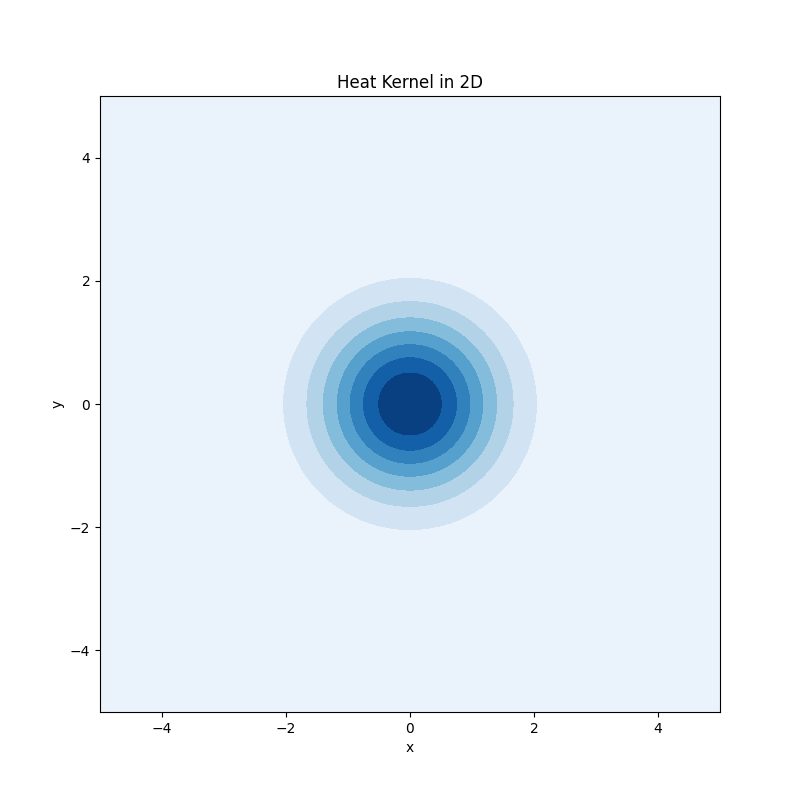
\includegraphics[width=0.5\textwidth]{figures/heat_kernel_2d.png}
            \end{figure}
            \begin{figure}
                \centering
                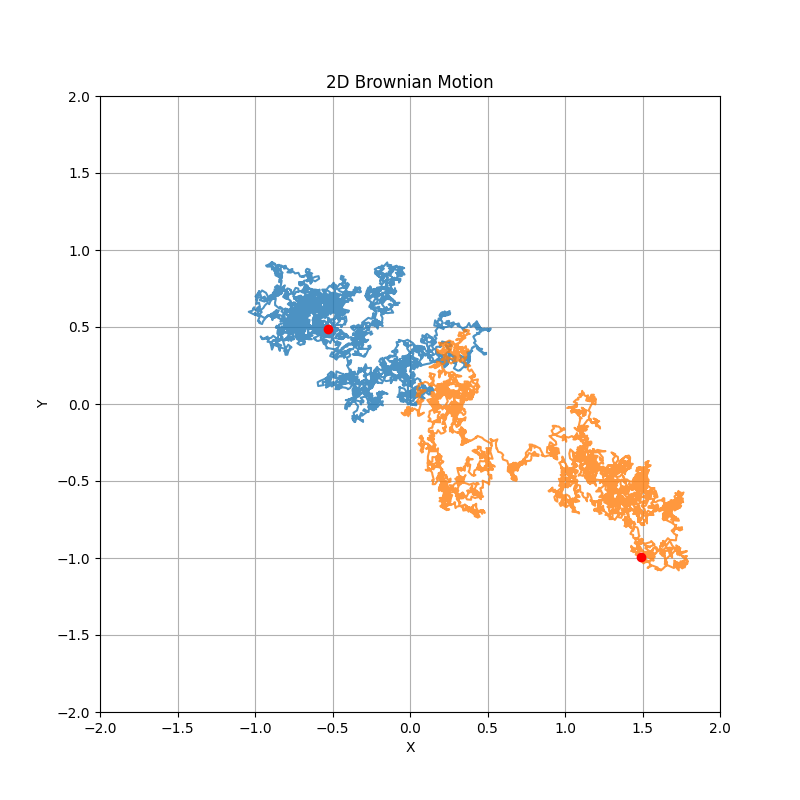
\includegraphics[width=0.5\textwidth]{figures/brownian_motion_2d.png}
            \end{figure}
        \end{column}
    \end{columns}
\end{frame}

\begin{frame}{A physical perspective}
    \begin{columns}
        \begin{column}{0.5\textwidth}
            \begin{block}{Heat semigroup}
                Time-evolution of a diffusion process, irreversible.
            \end{block}
            % space
            \vspace{1em}
            Ensemble Average
            \begin{equation*}
                \frac{1}{N} \sum_{i = 1}^N f(X^{(i)}_t) \xrightarrow{N \to \infty} \mathbb{E}[f(X_t)] = H_t f 
            \end{equation*}

            % space
            \vspace{1em}

            \begin{block}{Brownian Motion}
                Microscopic model of particles in heat motion, reversible.
            \end{block}
            
        \end{column}
        \begin{column}{0.5\textwidth}
            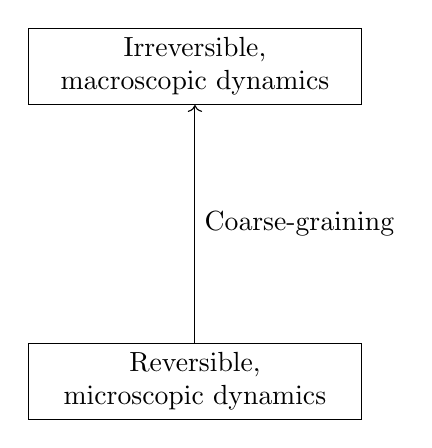
\begin{tikzpicture}
                \node (A) at (0,0) [draw, rectangle, text width=4cm, align=center] {Reversible,\\ microscopic dynamics};
                \node (B) at (0,4) [draw, rectangle, text width=4cm, align=center] {Irreversible,\\ macroscopic dynamics};
                \draw[->] (A) -- (B) node[midway, right] {Coarse-graining};
            \end{tikzpicture}
            
            
        \end{column}
    \end{columns}
\end{frame}

\begin{frame}{A physical perspective, cont.}
    \begin{columns}
        \begin{column}{0.5\textwidth}
            \begin{figure}
                \centering
                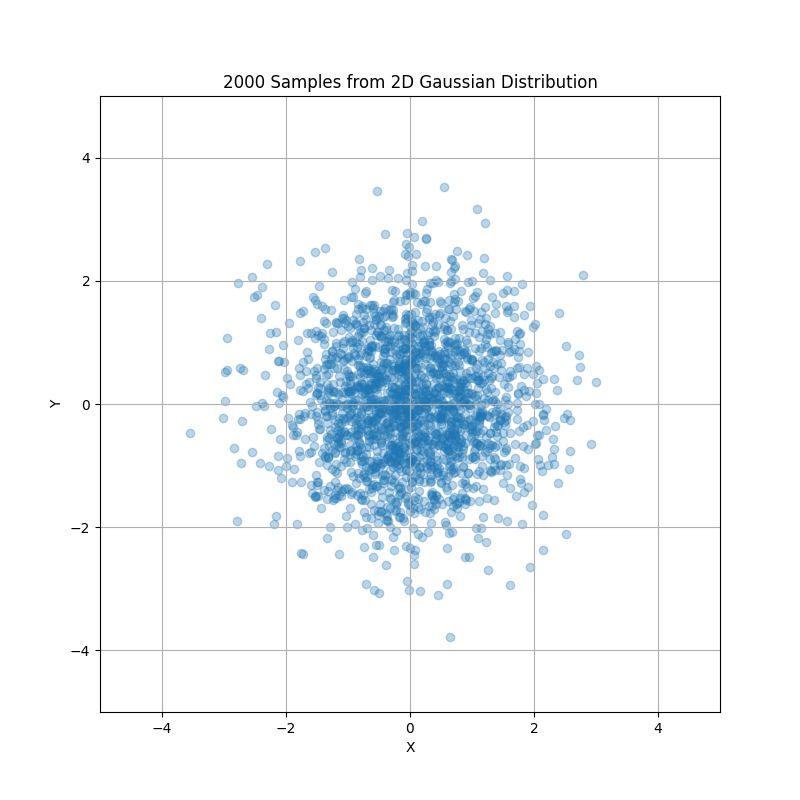
\includegraphics[width=\textwidth]{figures/gaussian_samples_2d.png}
                % \caption{Process 1}
            \end{figure}
        \end{column}
        \begin{column}{0.5\textwidth}
            \begin{figure}
                \centering
                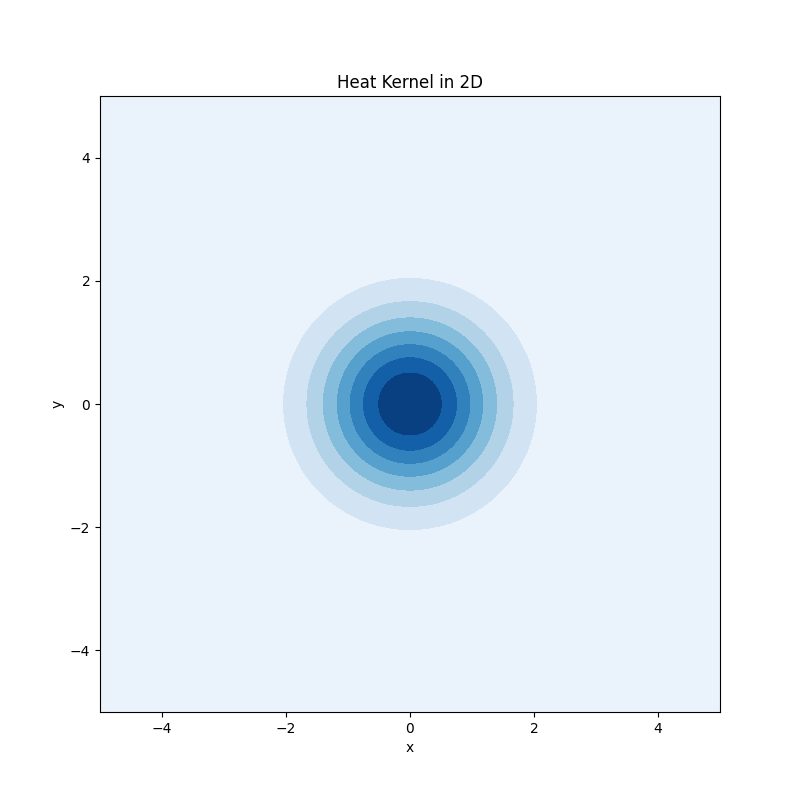
\includegraphics[width=\textwidth]{figures/heat_kernel_2d.png}
                % \caption{Process 2}
            \end{figure}
        \end{column}
    \end{columns}
\end{frame}





\section{Scaling Limit}
\begin{frame}{Scaling behavior in the non-interacting case}
    Consider $w(n) \equiv 1$. This is \textit{simple random walk}.
    
        \begin{minipage}{0.45\textwidth}
            \centering
            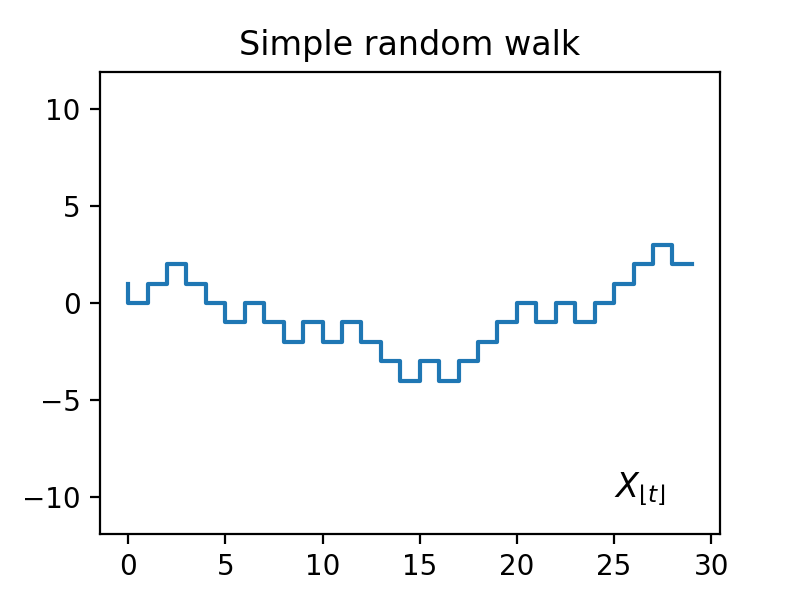
\includegraphics[width=\textwidth]{figures/srw_x1.png}<1>
            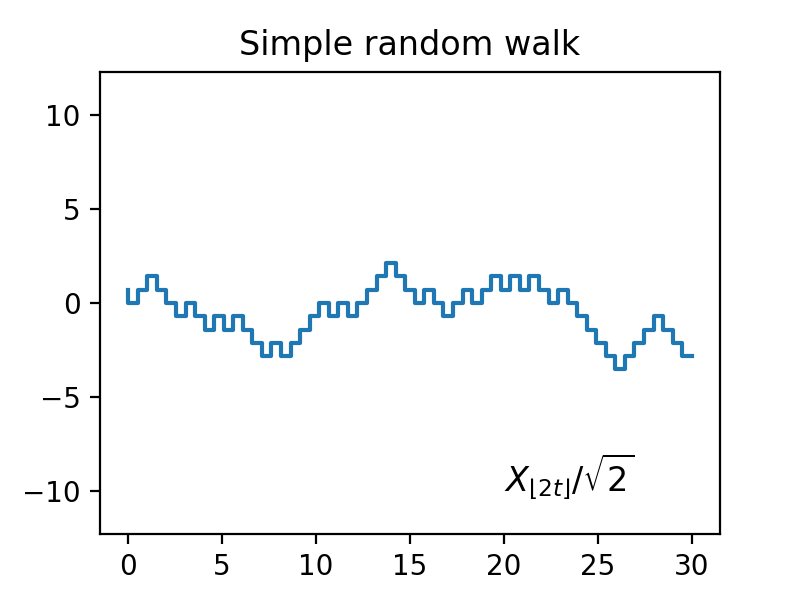
\includegraphics[width=\textwidth]{figures/srw_x2.png}<2>
            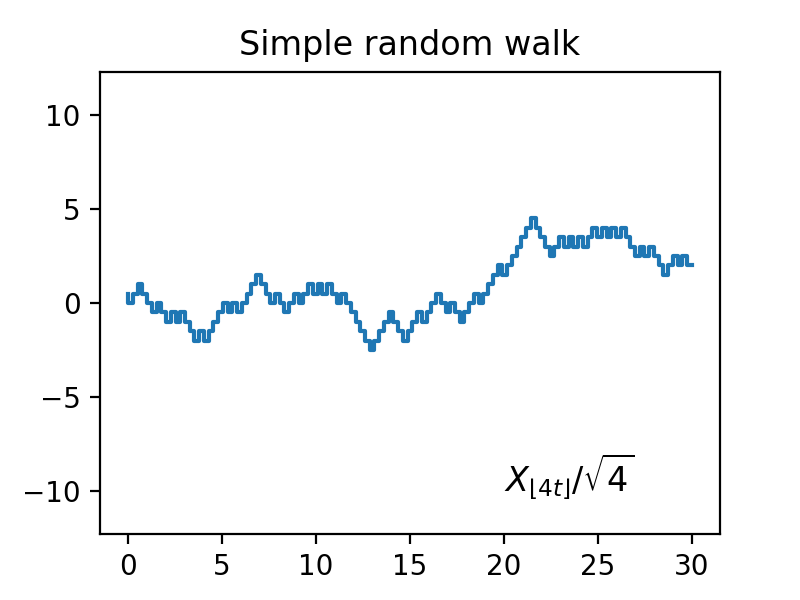
\includegraphics[width=\textwidth]{figures/srw_x3.png}<3>
            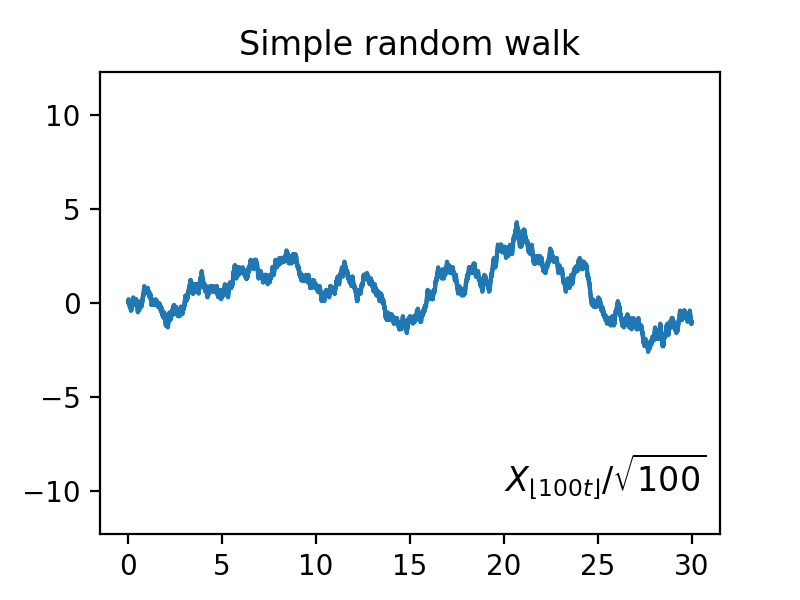
\includegraphics[width=\textwidth]{figures/srw_x4.png}<4->
        \end{minipage}
        \begin{math}
        \uncover<6->{\frac{X_{nt}}{\sqrt{n}} \xrightarrow{n \to \infty} B_t}
        \end{math}
        \begin{minipage}{0.45\textwidth}
            \centering
            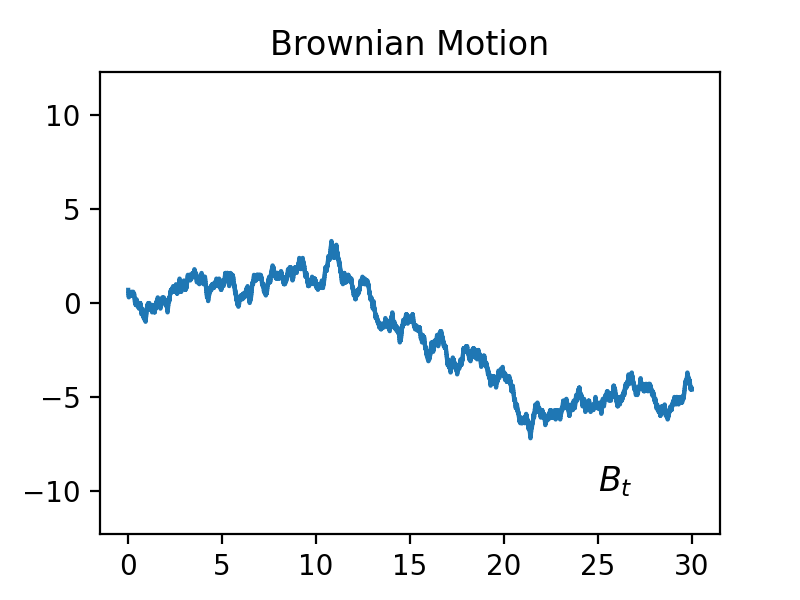
\includegraphics[width=\textwidth]{figures/srw_x5.png}<5->
        \end{minipage}
    % three parallel text blocks
    \begin{block}<7->{Good to know}
        \begin{columns}
            % 3 columns
            \begin{column}{0.3\textwidth}
                \begin{itemize}
                    \item 
                    $ B_t - B_s \sim \mathcal{N}(0, t-s)$
                    \item Markov process
                \end{itemize}
            \end{column}
            \begin{column}{0.3\textwidth}
                \begin{itemize}
                    \item $E(X_{t + s} | X_s) = X_s$
                    \item Martinagle
                \end{itemize}
            \end{column}
            \begin{column}{0.3\textwidth}
                \begin{itemize}
                    \item Visits every point infinitely often
                    \item Recurrent
                \end{itemize}
            \end{column}
        \end{columns}
    \end{block}

    \begin{alertblock}<8->{Question}
        How to understand self-interacting random walks in general?
    \end{alertblock}
\end{frame}

\section{Local Time}

\begin{frame}{Local Time Process}
    \begin{block}{Definition}
        \begin{itemize}
        \item $L(y, T)$, the \textbf{local time} of $X_k$ at site $y$ and time $T$, is the number of times the walk visits $y$ up to time $T$.

        \item $\mathcal{E}(y, T)$, the \textbf{directed edge local time}, is the number of times the walk traverses the edge $(y \to y+1)$ up to time $T$.

        \item $L(\cdot, T)$ and $\mathcal{E}(y, T)$ are random processes on $\mathbb{Z}^1$.
        \end{itemize}
        
    \end{block}

        % figure doodle-blp.png
        \begin{figure}
            \centering
            \includegraphics<1>[width=0.5\textwidth]{figures/doodle-blp.png}
            \includegraphics<2>[width=0.5\textwidth]{figures/doodle-blp2.png}
        \end{figure}

    \pause
    Let $\lambda_{x,m}$ be the time when the walk pays $m$-th visit to $x$.
    
    \begin{alertblock}{Observation}
    On event $\{T = \lambda_{x,m}\}$, the directed edge local time $\mathcal{E}(\cdot, T)$ is a Markov process.

    % It is very similar to a Branching Process.
    \end{alertblock}
\end{frame}

\begin{frame}{Identify scaling limit from local time process}
    The local time process $L(y, \lambda_{x, m})$ is much simpler, and carries scaling information of $X_k$.

    % four figures in two rows,
    \begin{figure}
        \centering
        \begin{minipage}{0.35\textwidth}
            \centering
            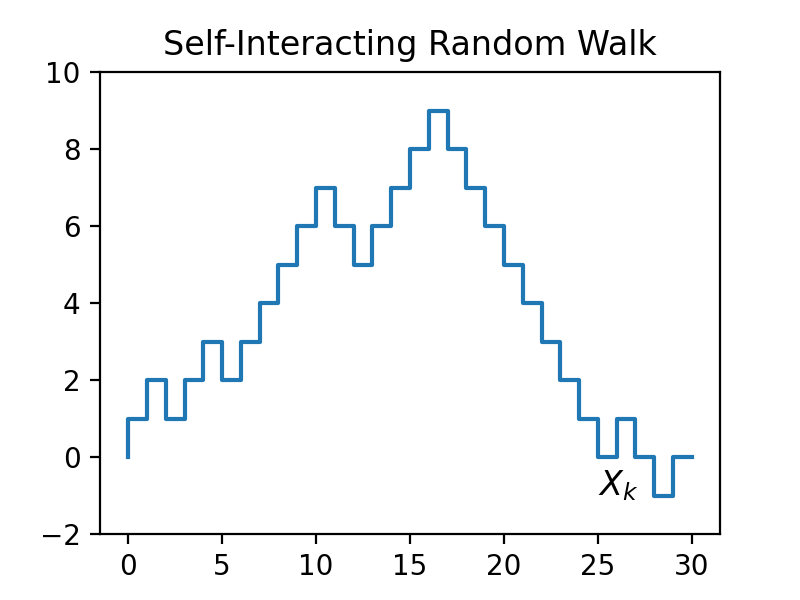
\includegraphics[width=\textwidth]{figures/sirw.png}
            \includegraphics<3->[width=\textwidth]{figures/sirwrescaled.png}
        \end{minipage}
        \begin{minipage}{0.35\textwidth}
            \centering
            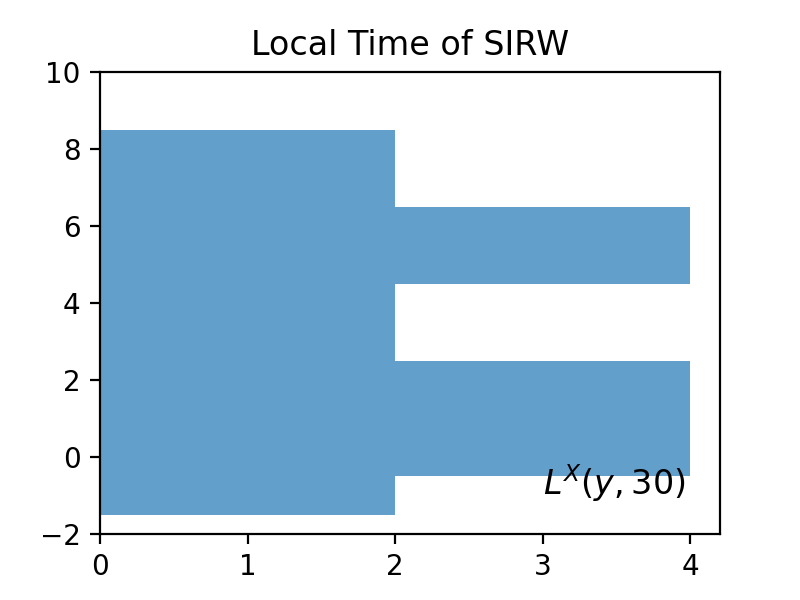
\includegraphics[width=\textwidth]{figures/sirwlocal.png}
            \includegraphics<2->[width=\textwidth]{figures/sirwlocalrescaled.png}
        \end{minipage}
    \end{figure}
\end{frame}
\begin{frame}{Identify scaling limit from local time process}
    \begin{block}{Conjecture (Toth, 1996)}
        If $w(n)$ satisfies certain conditions, then $X_k$ converges after scaling to a Brownian motion perturbed at extrema $W_t$, defined by
        \begin{equation}
            W_t = B_t + \gamma_w (\sup_{s \leq t} W_s + \inf_{s \leq t} W_s)
        \end{equation}
    \end{block}


\end{frame}

\section{Our Results}

\begin{frame}{Our Results}
    \begin{block}{Theorem (Kosygina, Mountford and Peterson, 2023)}
        The convergence $X_k \to W_t$ holds for $w(n)$ satisfying
        \begin{equation*}
            \frac{1}{w(n)}=1+\frac{2^p B}{n^p}+O\left(\frac{1}{n^{1+\kappa}}\right) \quad \text{for some } p\in (\frac{1}{2}, 1], \kappa>0
        .\end{equation*}
    \end{block}
    \pause
    For smaller $p$ there were technical difficulties, resolved in the following theorem.
    \pause
    \begin{block}{Theorem (Liu and Wang, 2024)}
        The previous theorem can be generalized to $p \in (0,1]$.
    \end{block}
    \pause
    \begin{exampleblock}{In search of a general correspondence}
        \begin{minipage}{0.45\textwidth}
% https://quiver.local:8080/#q=WzAsNCxbMCwwLCJYXnsobil9Il0sWzIsMCwiTChYXnsobil9KSJdLFsyLDIsIkwoWSkiXSxbMCwyLCJZIl0sWzAsMV0sWzEsMl0sWzAsMywiIiwyLHsic3R5bGUiOnsiYm9keSI6eyJuYW1lIjoiZGFzaGVkIn19fV0sWzMsMl1d
\[\begin{tikzcd}[ampersand replacement=\&,cramped]
	{X^{(n)}} \&\& {L(X^{(n)})} \\
	\\
	Y \&\& {L(Y)}
	\arrow[from=1-1, to=1-3]
	\arrow[from=1-3, to=3-3]
	\arrow[dashed, from=1-1, to=3-1]
	\arrow[from=3-1, to=3-3]
\end{tikzcd}\]
\end{minipage}
\begin{minipage}{0.45\textwidth}

What precise conditions are necessary to pass from local time convergence to the convergence of the processes themselves?
\end{minipage}
    \end{exampleblock}

        
\end{frame}

\begin{frame}{Main Ideas}
    \begin{itemize}
        \item \emph{Random walks} with \emph{local interactions} help us understand complex physical systems that are important in statistical mechanics.
        \item \emph{Scaling limit} can bring a discrete process on $\mathbb{Z}^1$ to a continuous process on $\mathbb{R}$.
        \item \emph{Local time process} carries information about the scaling limit of the random walk, if it exists.
        \item It would be interesting to understand the general correspondence between the convergence of the local time processes and the convergence of the random walks.
    \end{itemize}
\end{frame}

\section{References and Appendix}
\begin{frame}
    \begin{center}
        \Huge Questions?
    \end{center}
\vfill
    
\begin{itemize}
\item
    B\'{a}lint T\'{o}th, \emph{Generalized {R}ay-{K}night theory and limit theorems for self-interacting random walks on {${\bf Z}^1$}}, Ann. Probab. \textbf{24} (1996), no.~3, 1324--1367. \MR{1411497}

    \item
    Elena Kosygina, Thomas Mountford, and Jonathon Peterson,  \emph{Convergence and nonconvergence of scaled self-interacting random walks to {B}rownian motion perturbed at extrema}, Ann. Probab. \textbf{51} (2023), no.~5, 1684--1728. \MR{4642221}

    \item
    Patrick Billingsley, \emph{Convergence of probability measures}, second ed., Wiley Series in Probability and Statistics: Probability and Statistics, John Wiley \& Sons, Inc., New York, 1999, A Wiley-Interscience Publication. \MR{1700749}

    \item
    Xiaoyu Liu and Zhe Wang, \emph{Convergence of self-interacting random walks to Brownian Motion perturbed at extrema}, arXiv:2402.11828.

    \end{itemize}
\end{frame}

\begin{frame}
    \begin{block}{Theorem (KMP23)(LW24)}
        The convergence $X_k \to W_t$ holds for $w(n)$ satisfying
        \begin{equation*}
            \frac{1}{w(n)}=1+\frac{2^p B}{n^p}+O\left(\frac{1}{n^{1+\kappa}}\right) \quad \text{for some } p\in (0, 1], \kappa>0
        .\end{equation*}
    \end{block}
    \begin{block}{Theorem (KMP23)}
        The ``polynomial self-repelling'' SIRW, defined by
            $w(n)=(n+1)^{-\alpha}$
        does not converge in process level to BMPE. 
        (Finite-dimensional distributions are also unknown.)
    \end{block}
    \begin{exampleblock}{Open Problem}
        What precise conditions are necessary to pass from local time convergence to the convergence of the processes themselves?
    \end{exampleblock}
\end{frame}


% \begin{frame}{Proving $w$-SIRW $\implies$ BMPE}
%     \begin{block}{Proof Strategy}
%         \begin{enumerate}
%             \item Prove the extremal processes $\sup_{s \leq t} W_s$ and $\inf_{s \leq t} W_s$ are \textit{tight}.
%             \item Decompose $X_k$ into a \textit{martingale} part $M_k$ and a \textit{drift} part $\Gamma_k = \sum_{i = 0}^{k- 1} E[X_{i + 1} - X_i | \mathcal{F}_i^X]$.
%             \item Apply Martingale Central Limit Theorem to $M_k$. By controlling quadratic variation, show that $M_k$ converges to a Brownian motion.
%             \item Control the drift term:
%             \begin{equation*}
%                 \lim _{n \rightarrow \infty} \mathbb{P}\left(\sup _{k \leq\lfloor n t\rfloor}\left|\Gamma_k-\gamma \cdot\left(S_k + I_k\right)\right|>\varepsilon \sqrt{n}\right)=0
%             \end{equation*}
%             \item Those imply that $X_k$ converges to BMPE.
%         \end{enumerate}
%     \end{block}

% \end{frame}

\end{document}
